\subsection{组合模式(Composite)}

\subsubsection{组合模式简介}
组合模式是一种设计模式,它允许一组对象被当作单个对象对待。这样,用户可以对单个对象和组合对象进行相同的操作,无需关心它们是单个对象还是组合对象。

组合模式的主要用途是让用户对单个对象和组合对象进行相同的操作,而无需关心它们是否为组合对象。这样,用户可以更方便地管理一个对象层次结构,并对其进行操作。

例如,在文件系统中,一个文件夹可以包含多个文件和子文件夹。使用组合模式,用户可以对文件夹和文件进行相同的操作,比如查看、删除和复制。无需关心它们是文件夹还是文件,就可以对它们进行统一的处理。

组合模式的优点包括:
\begin{enumerate}
    \item 统一了对象层次结构:组合模式可以将单个对象和组合对象进行统一,让用户可以对它们进行相同的操作。
    \item 方便对对象层次结构的管理:使用组合模式,用户可以方便地管理一个对象层次结构,并对其进行操作。
    \item 增加系统的灵活性:组合模式可以让用户在运行时动态地组合对象,增加系统的灵活性。
\end{enumerate}

组合模式的缺点包括:

\begin{enumerate}
    \item 增加系统的复杂度:组合模式可能会增加系统的复杂度,因为它需要设计一个组合类来管理单个对象和组合对象。
    \item 可能会过度抽象:如果组合类的接口过于抽象,可能会导致用户难以理解和使用它。
    \item 可能会掩盖组合对象的问题:如果组合对象存在问题,组合模式可能会掩盖这些问题,导致用户无法及时发现并解决问题。
\end{enumerate}

\subsubsection{组合模式在项目中的应用}

\begin{figure}[h]
    \centering
    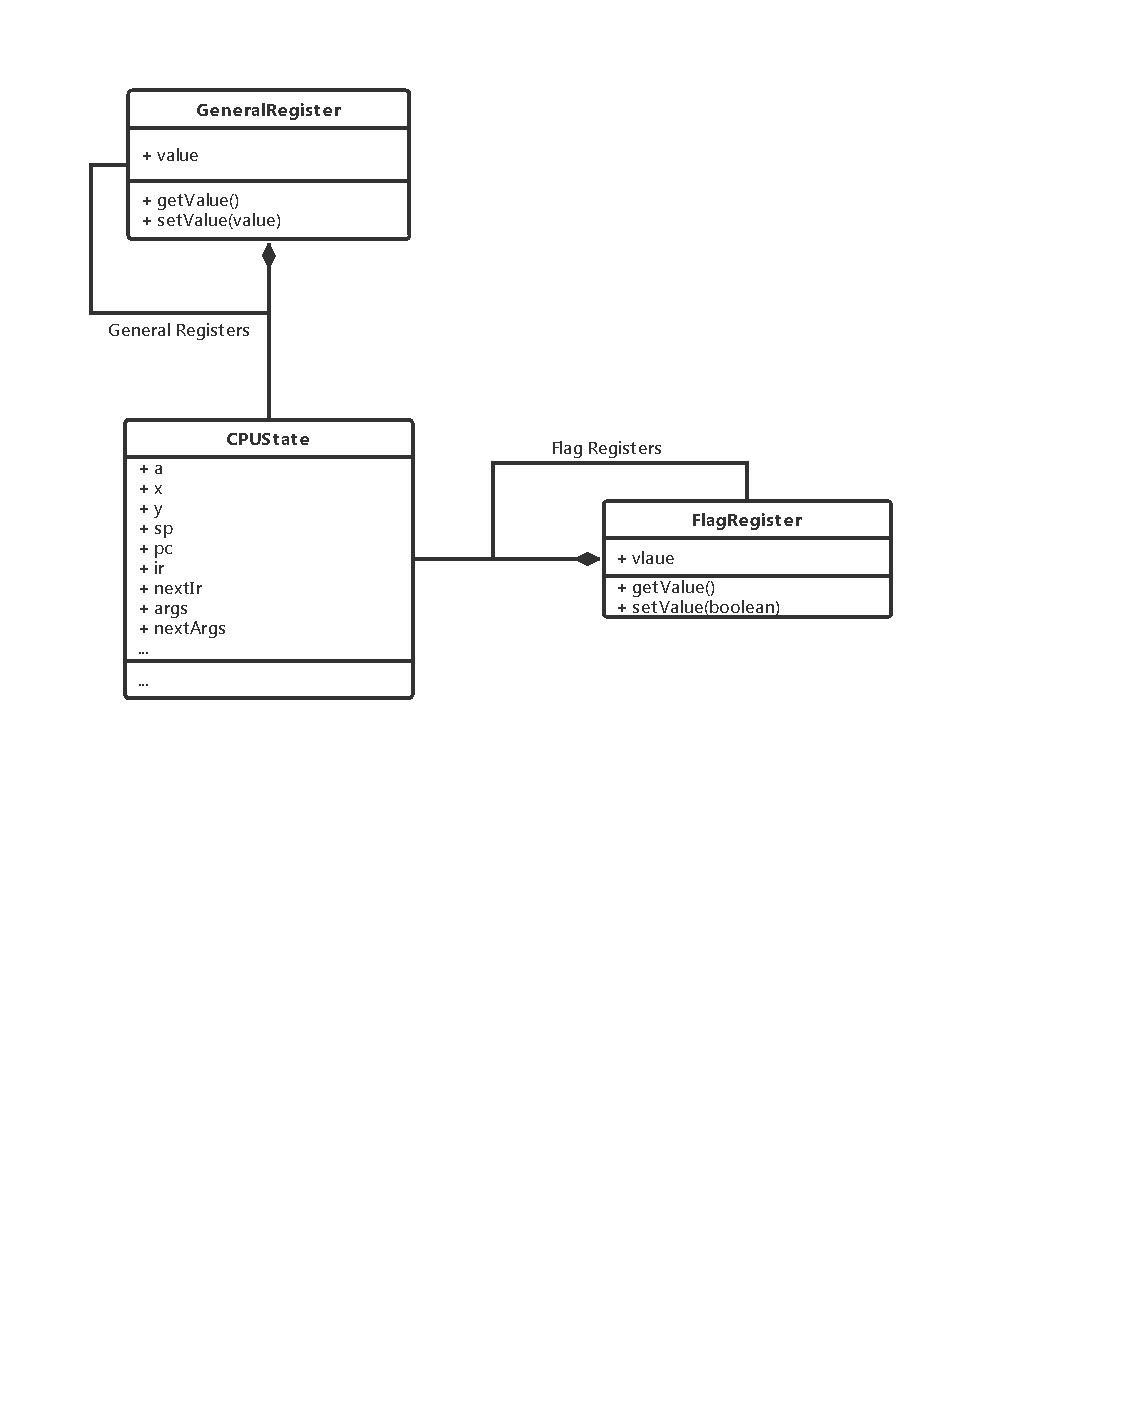
\includegraphics[width=0.9\textwidth]{figures/Composite.pdf}
    \caption{组合模式在 Slow6502 中的类图}
\end{figure}

在我们的项目中,我们使用组合模式构建使用的 CPU State 。由于 CPU State 中包含大量不同的更小的组成部分(寄存器、状态位)等,故而使用组合模式可方便地管理 CPU State 的层次结构,并对其进行操作。

